% header
\documentclass[10pt,a4paper]{article}

\usepackage[utf8]{inputenc}
\usepackage{hyperref}
\usepackage{amssymb}
\usepackage{amsmath}
\usepackage{listings}
\usepackage{graphicx}

% the document
\begin{document}

\title{Worksheet $4$\\
\small{Practical Lab Numerical Computing}}
\author{Andrii Lischishin \and Lars Schleithoff \and Hendrik Kleikamp}
\date{\today}
\maketitle

\section*{Task 1}

\begin{center}
	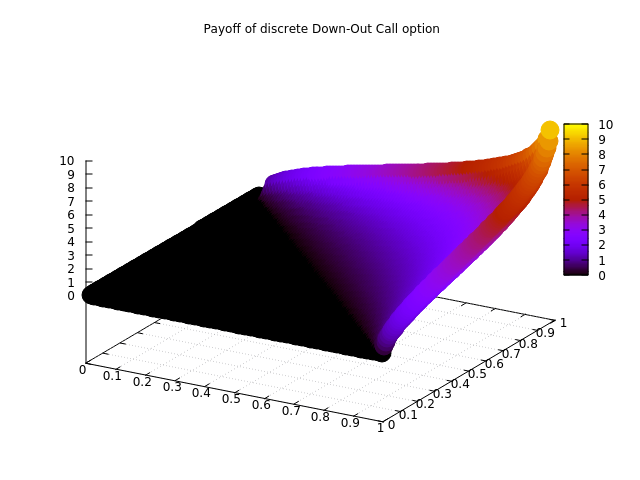
\includegraphics[scale=0.7]{payoff_down_out_call.png}
\end{center}

\section*{Task 2}


\begin{center}
	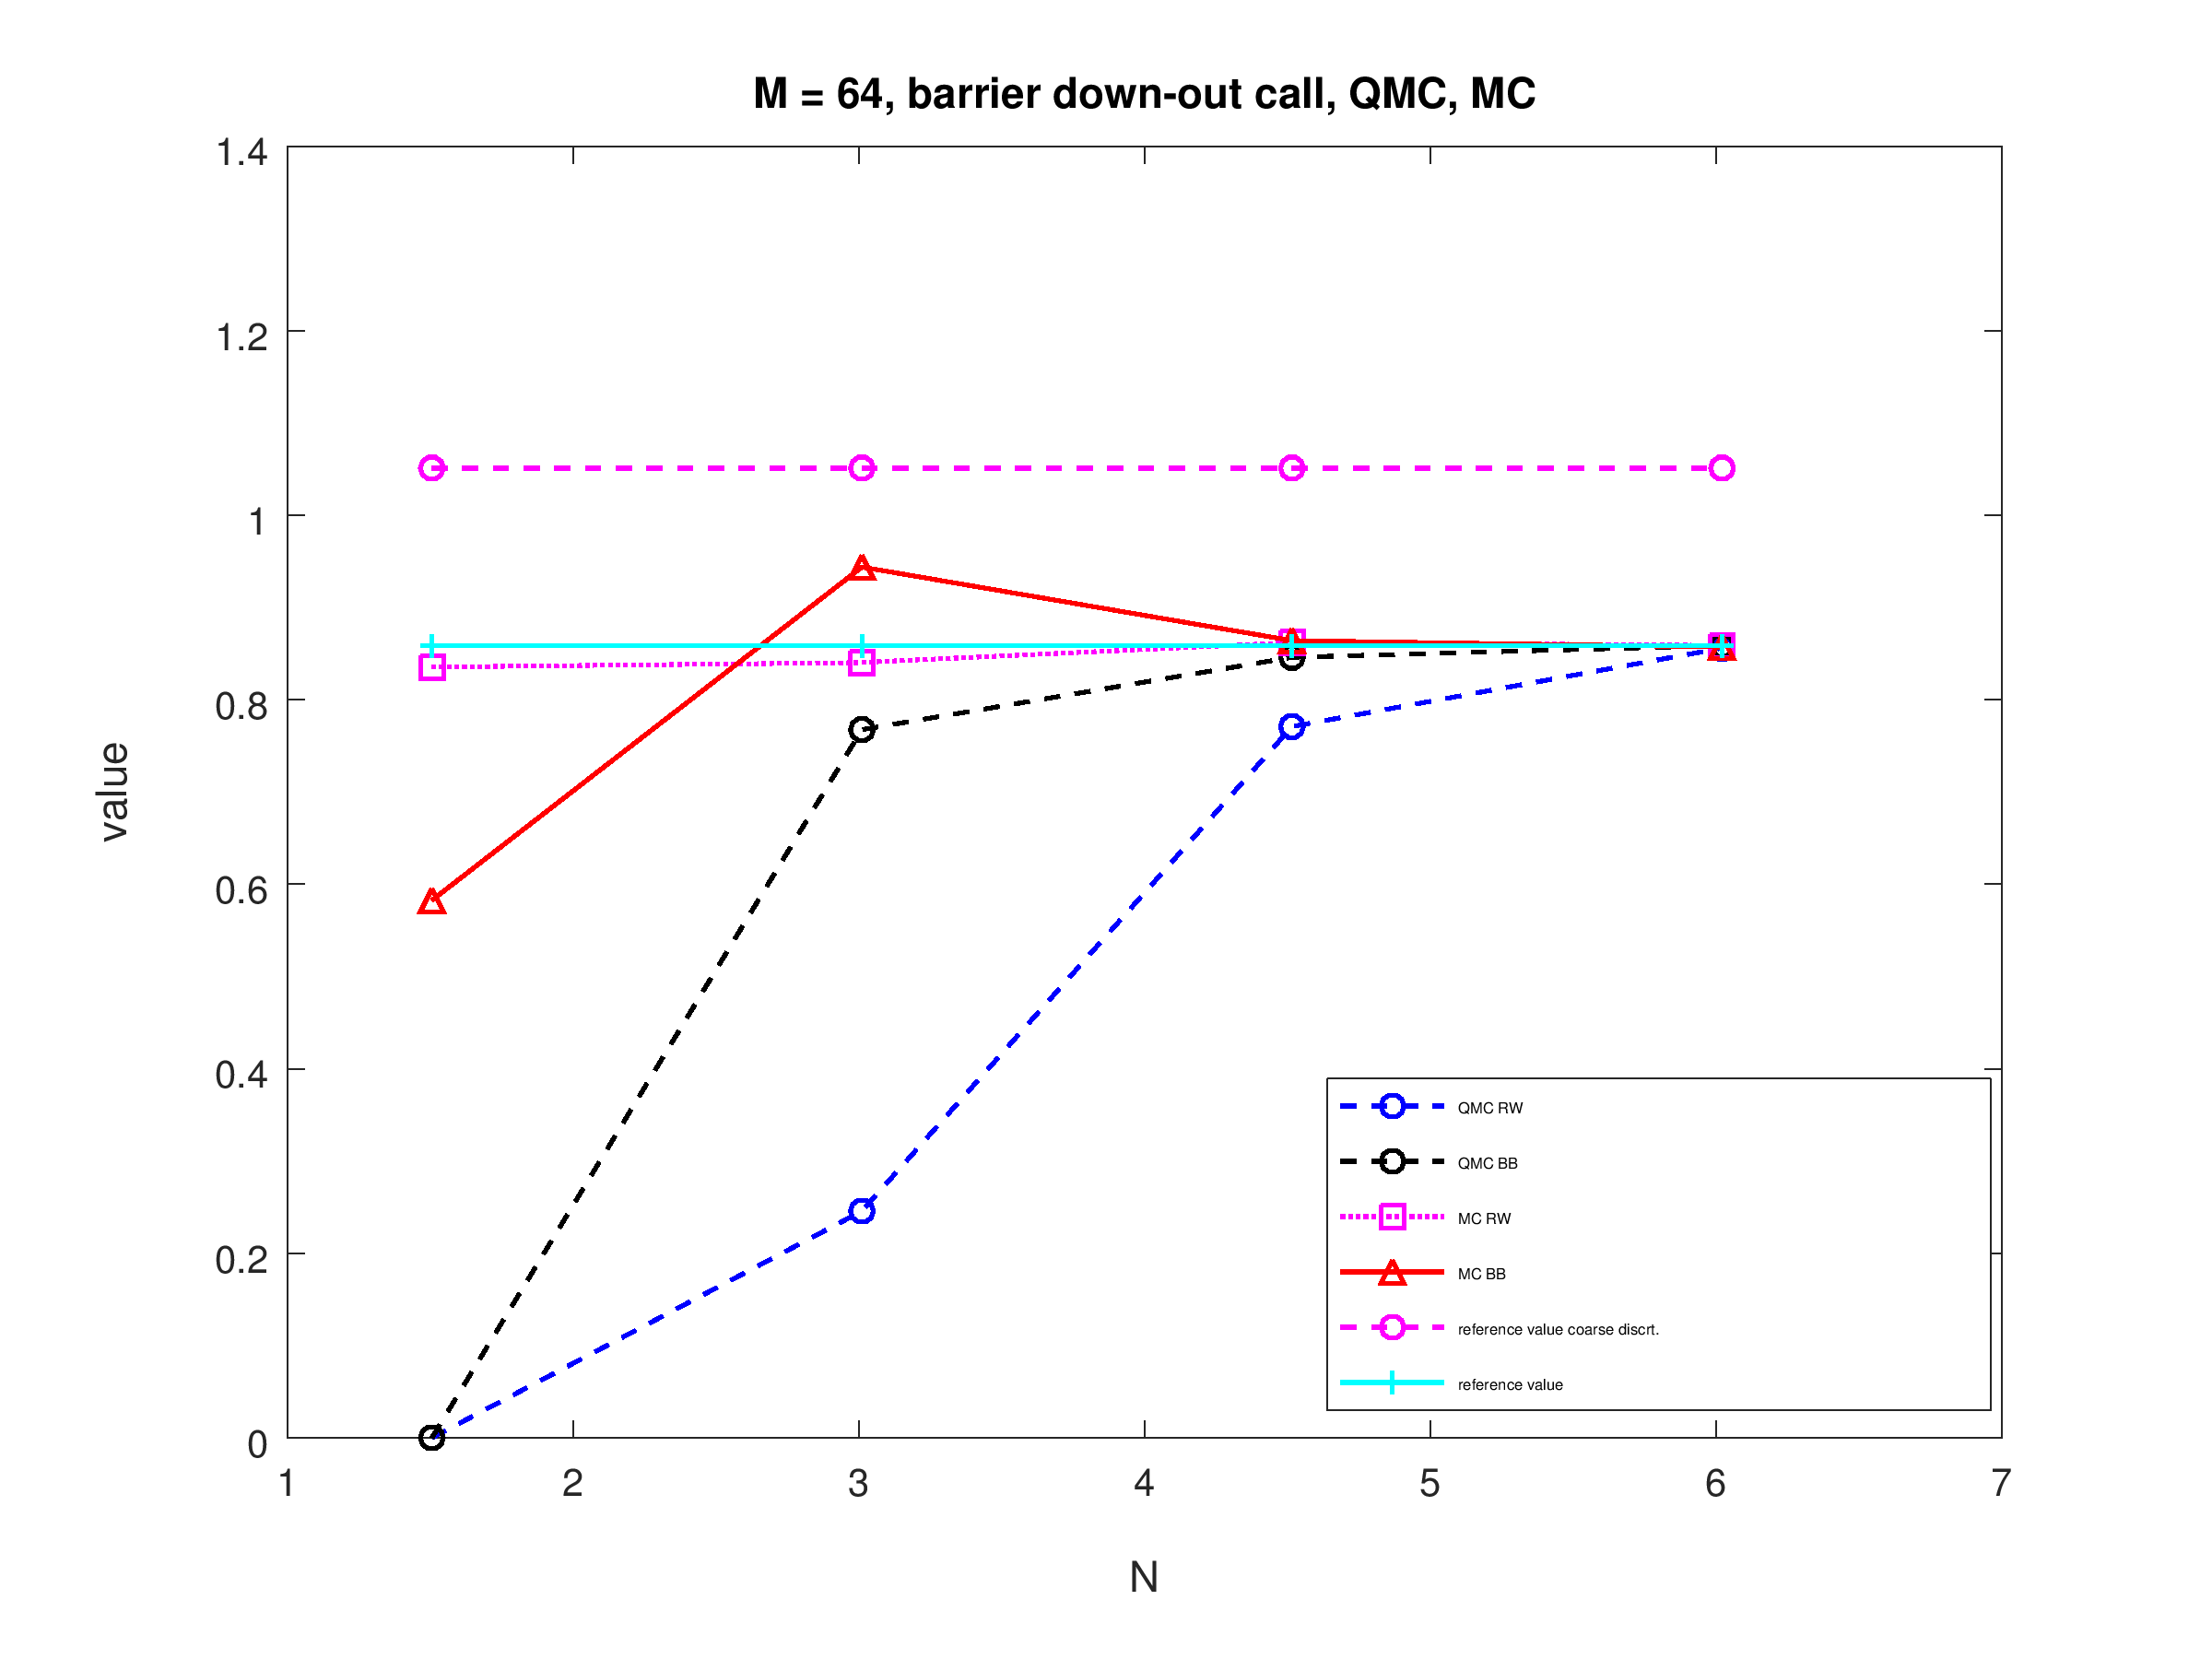
\includegraphics[scale=0.35]{../image/task2.png}
\end{center}

\begin{itemize}
    \item{On this figure value of barrier Down-Out Call option using different methods is plotted against number of used points($10^N$).
    }
\item{
Pink dashed line is reference value which you get, if precision is too low. So, if precision is too low then reference value lies above or below the actual price.
}
\item{
From the plots, one can observe that for QMC Brownian-Bridge shows quicker convergence than Random-Walk, but for MC it is vice verse.
}
\end{itemize}
Next figure represents error convergence-rates of the above figure.

\begin{center}
	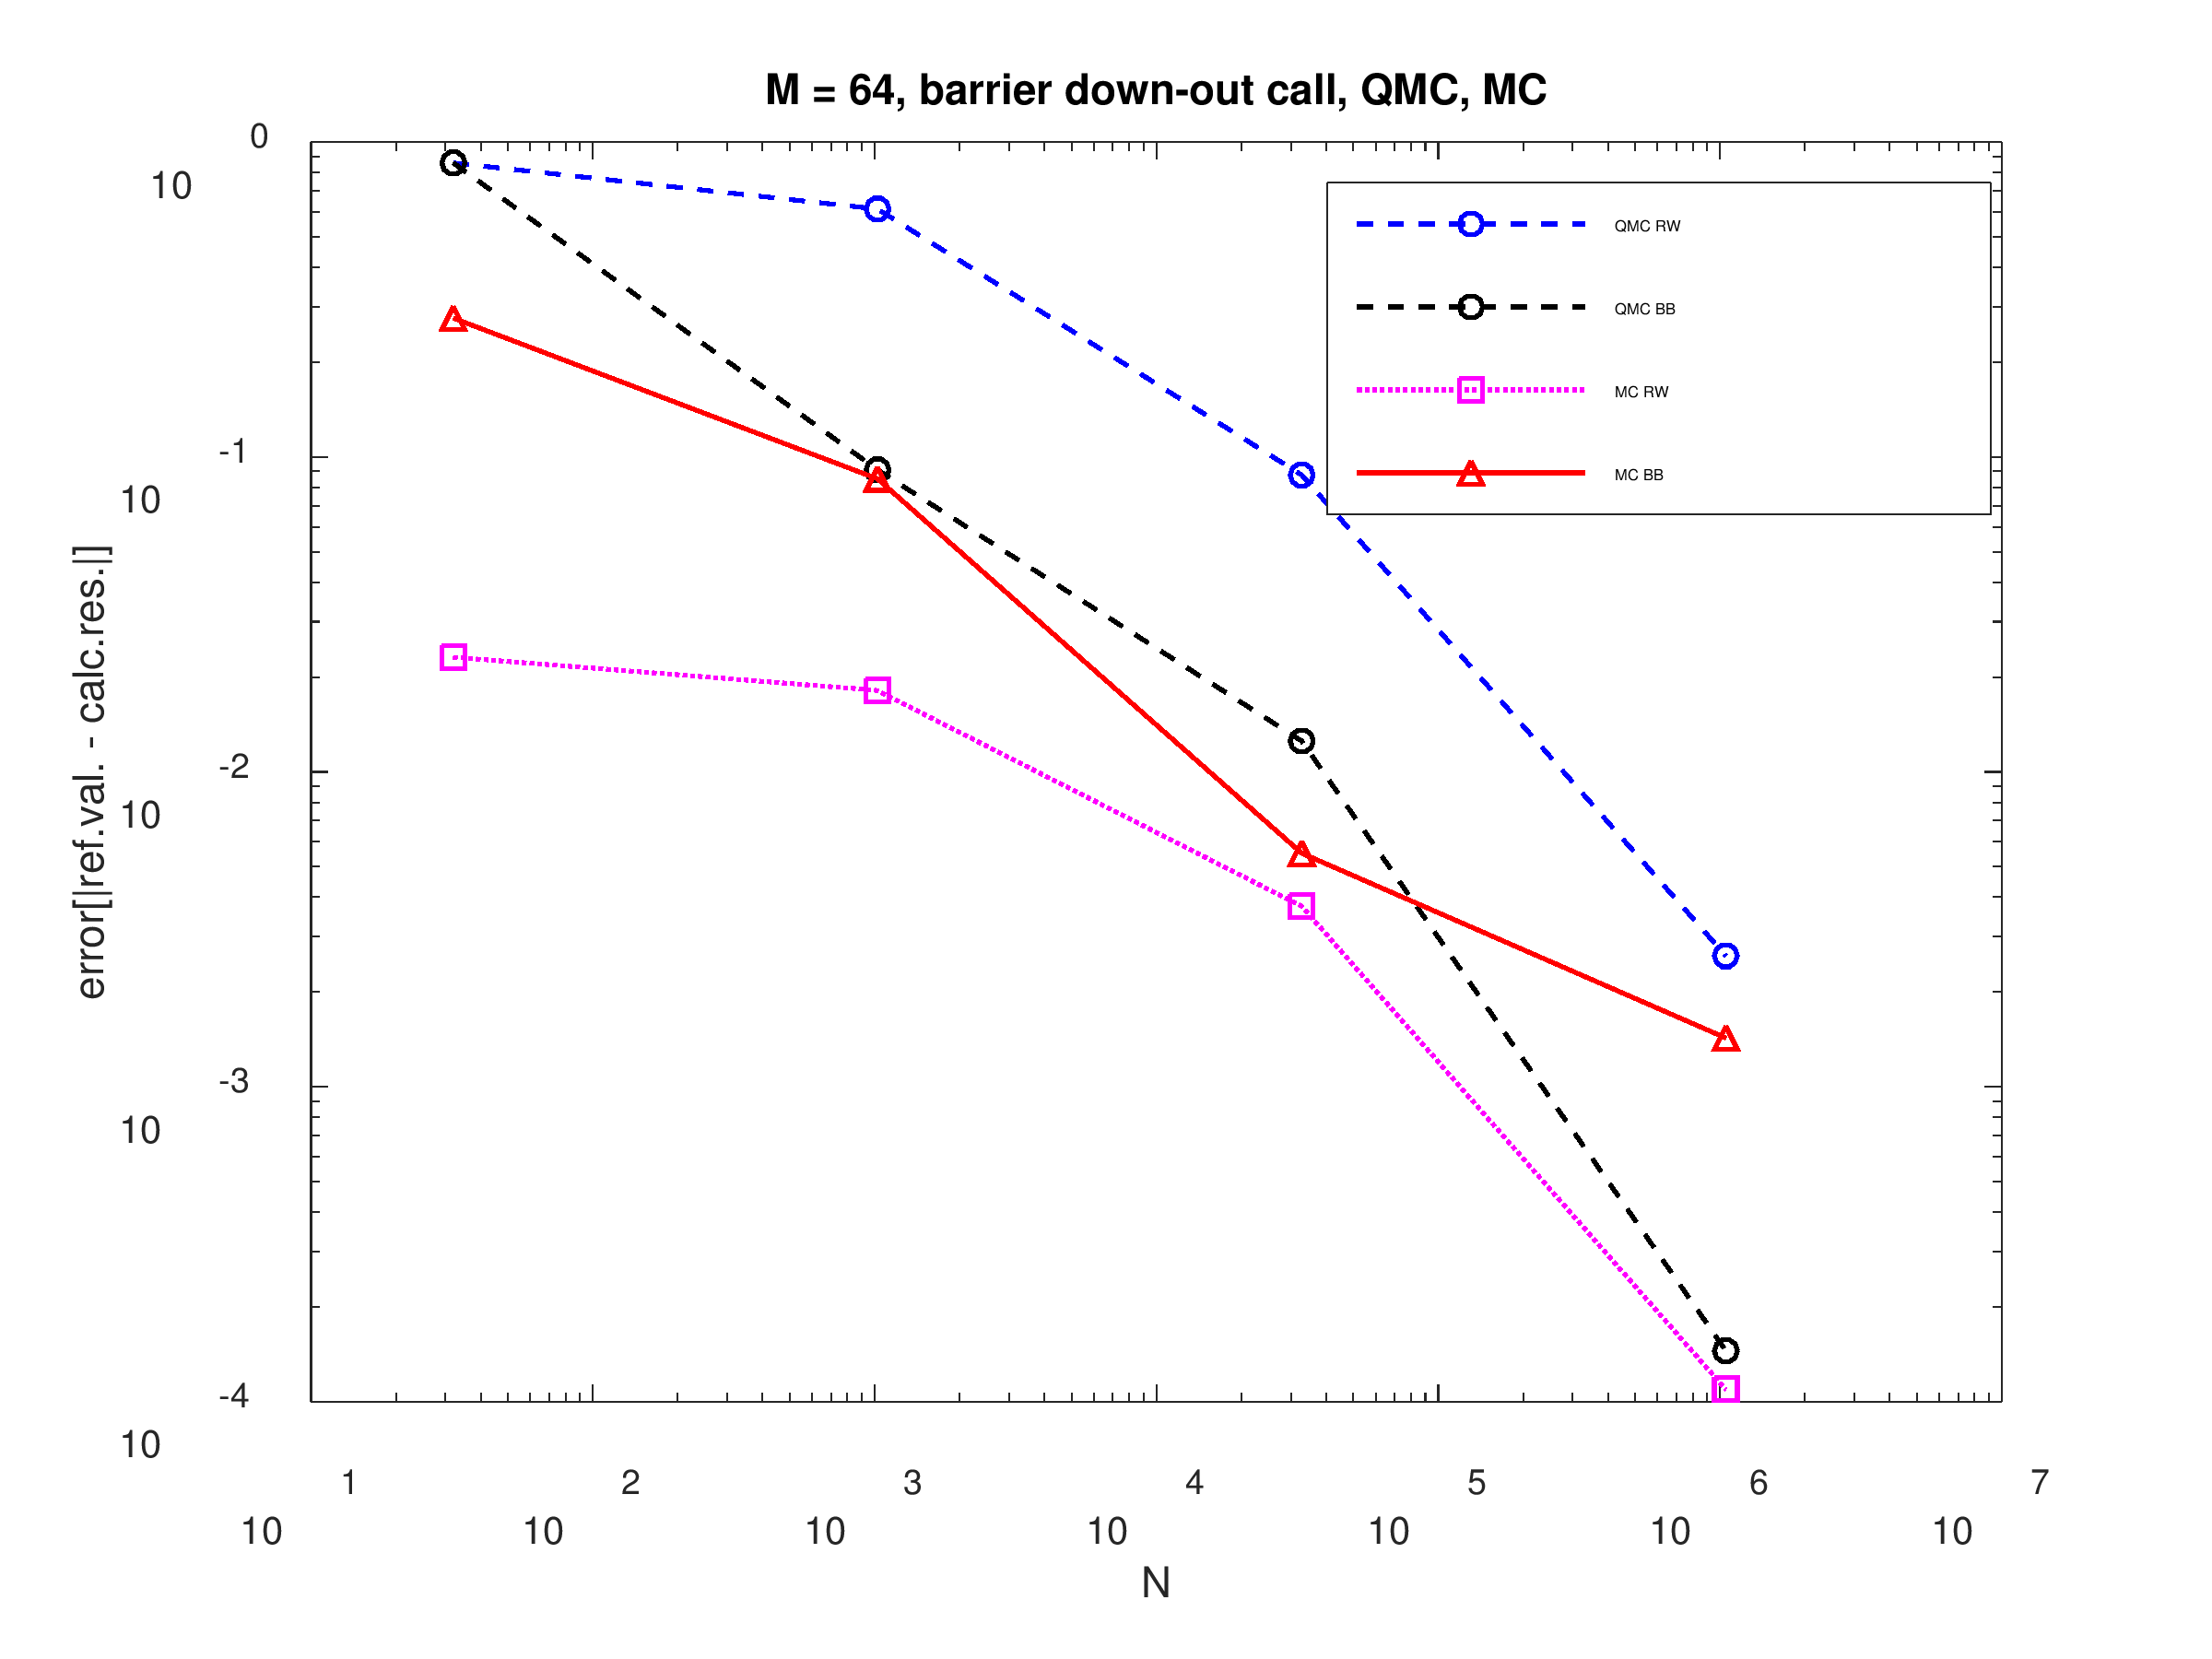
\includegraphics[scale=0.35]{../image/task2_error.png}
\end{center}

\section*{Task 3}

\begin{center}
	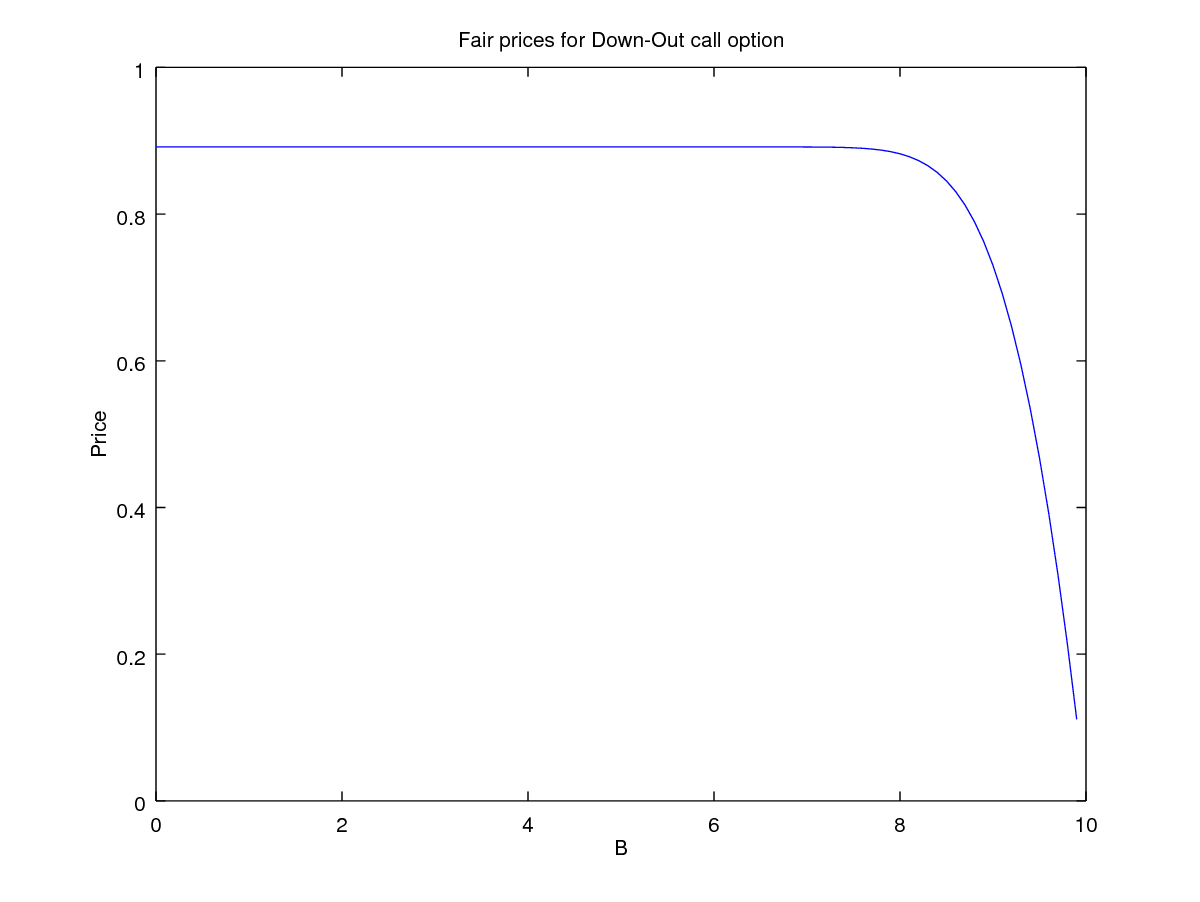
\includegraphics[scale=0.7]{fair_prices_down_out_call.png}
\end{center}

\section*{Task 4}

\begin{center}
	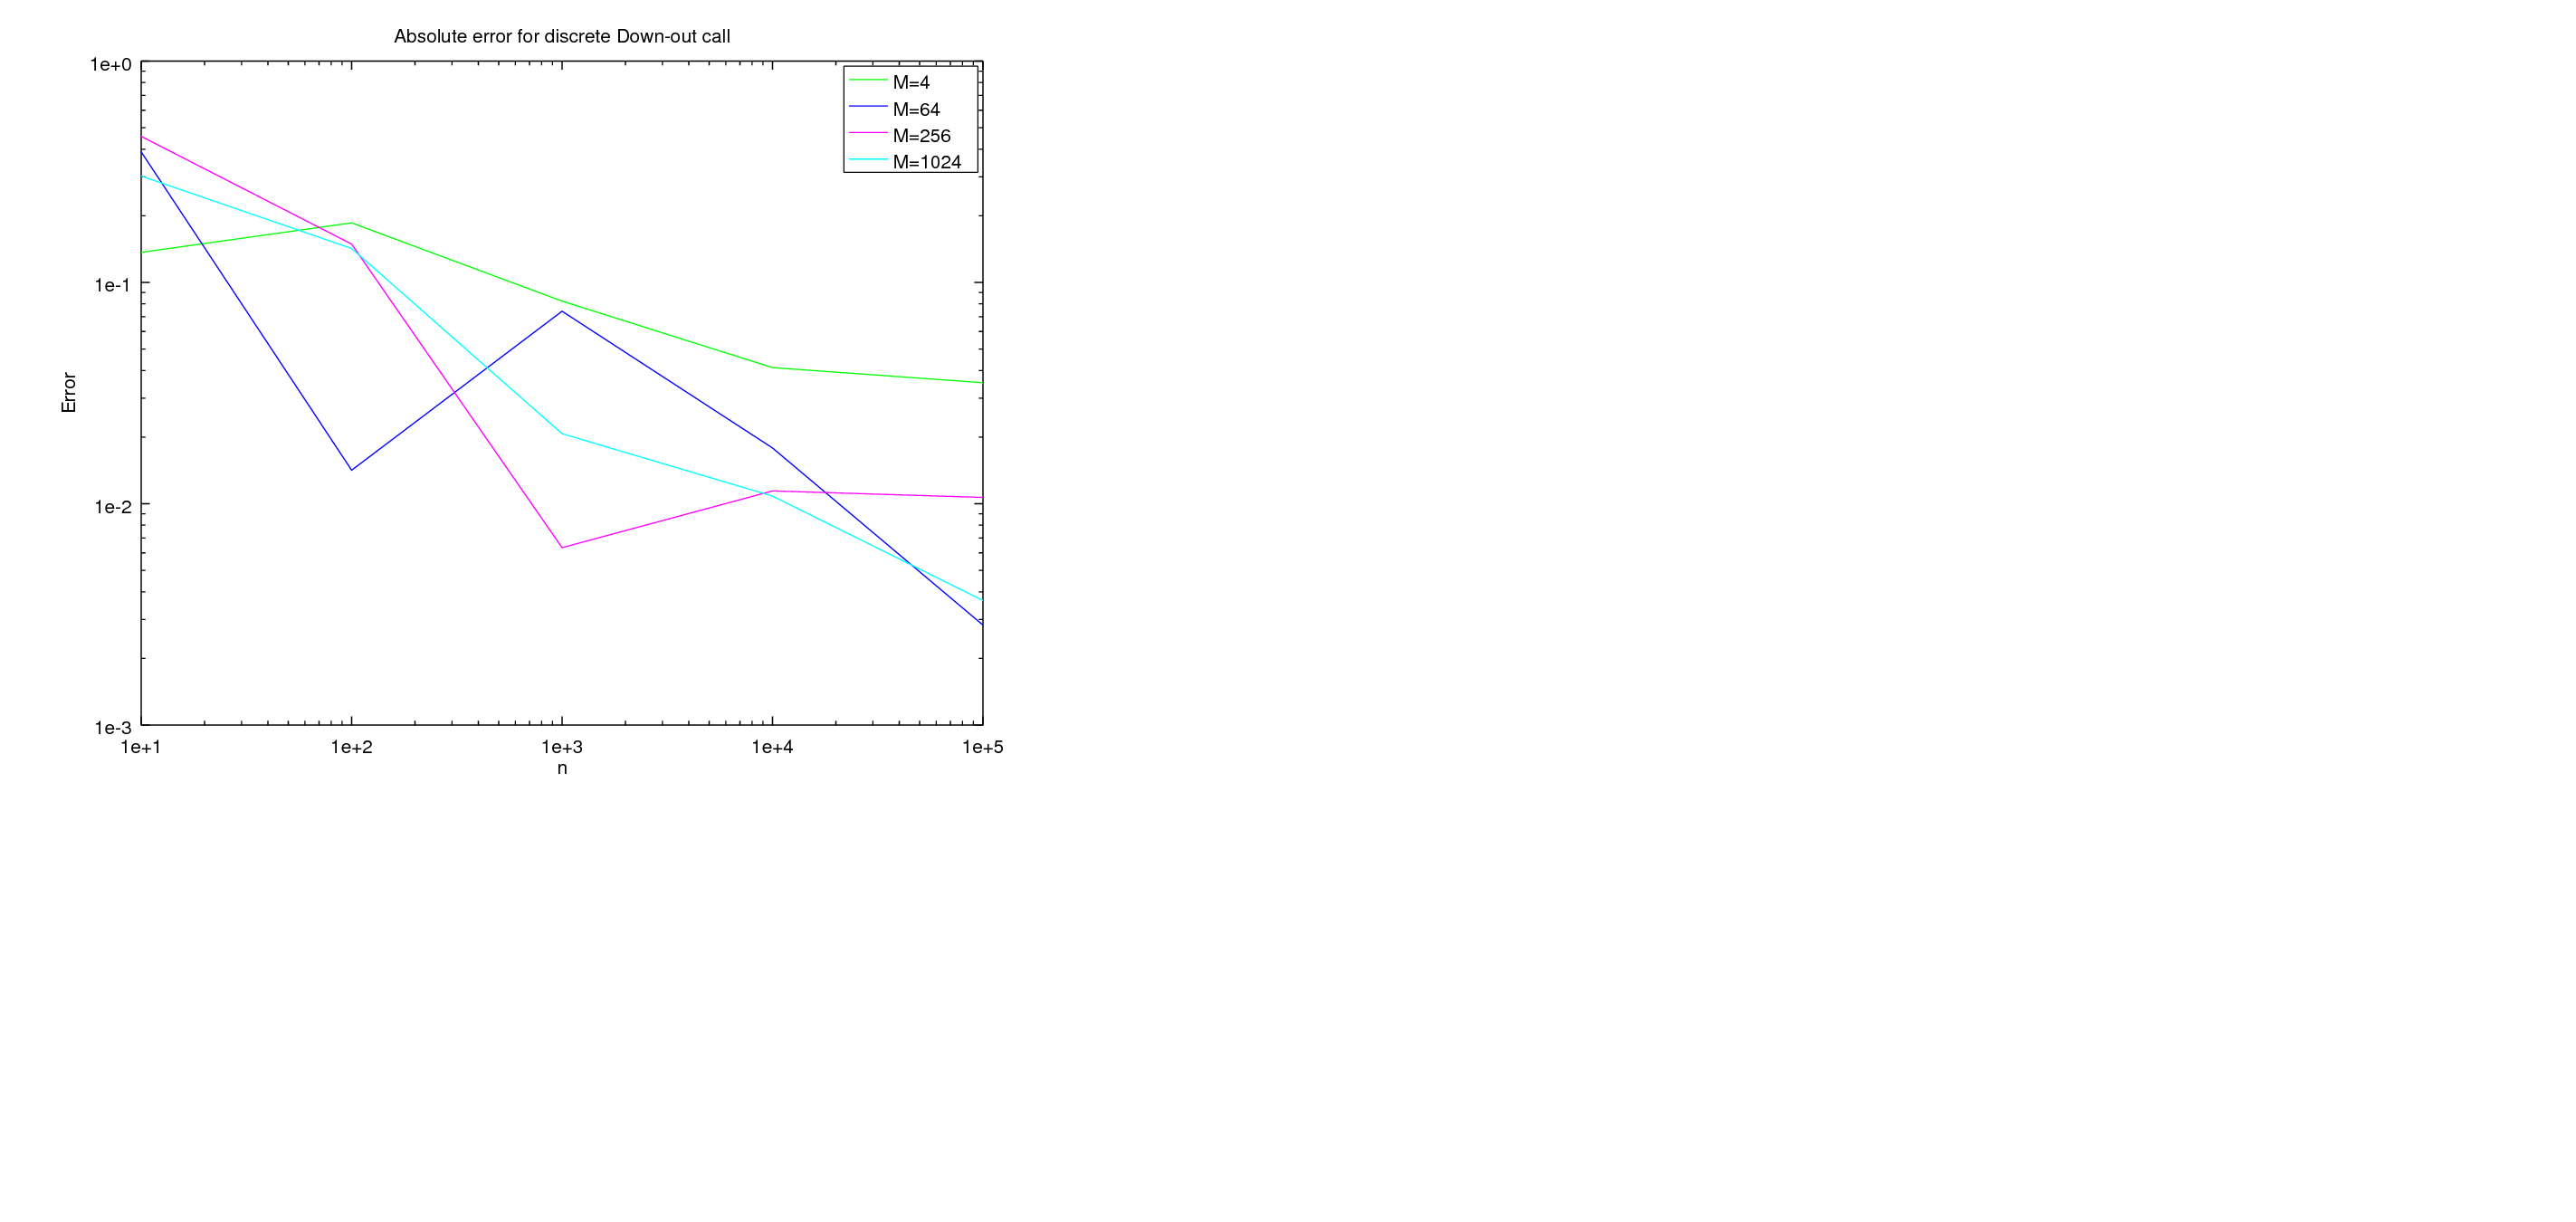
\includegraphics[scale=0.7]{convergence_plot_discrete_down_out_call.png}
\end{center}

\section*{Task 5}

\begin{center}
	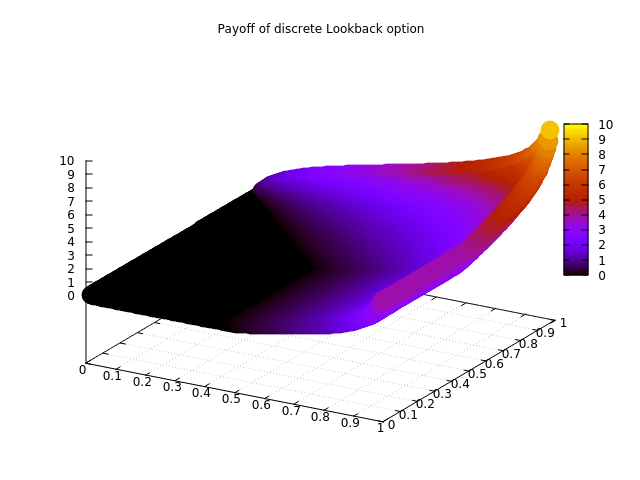
\includegraphics[scale=0.7]{payoff_lookback.png}
\end{center}

\section*{Task 6}

\begin{center}
	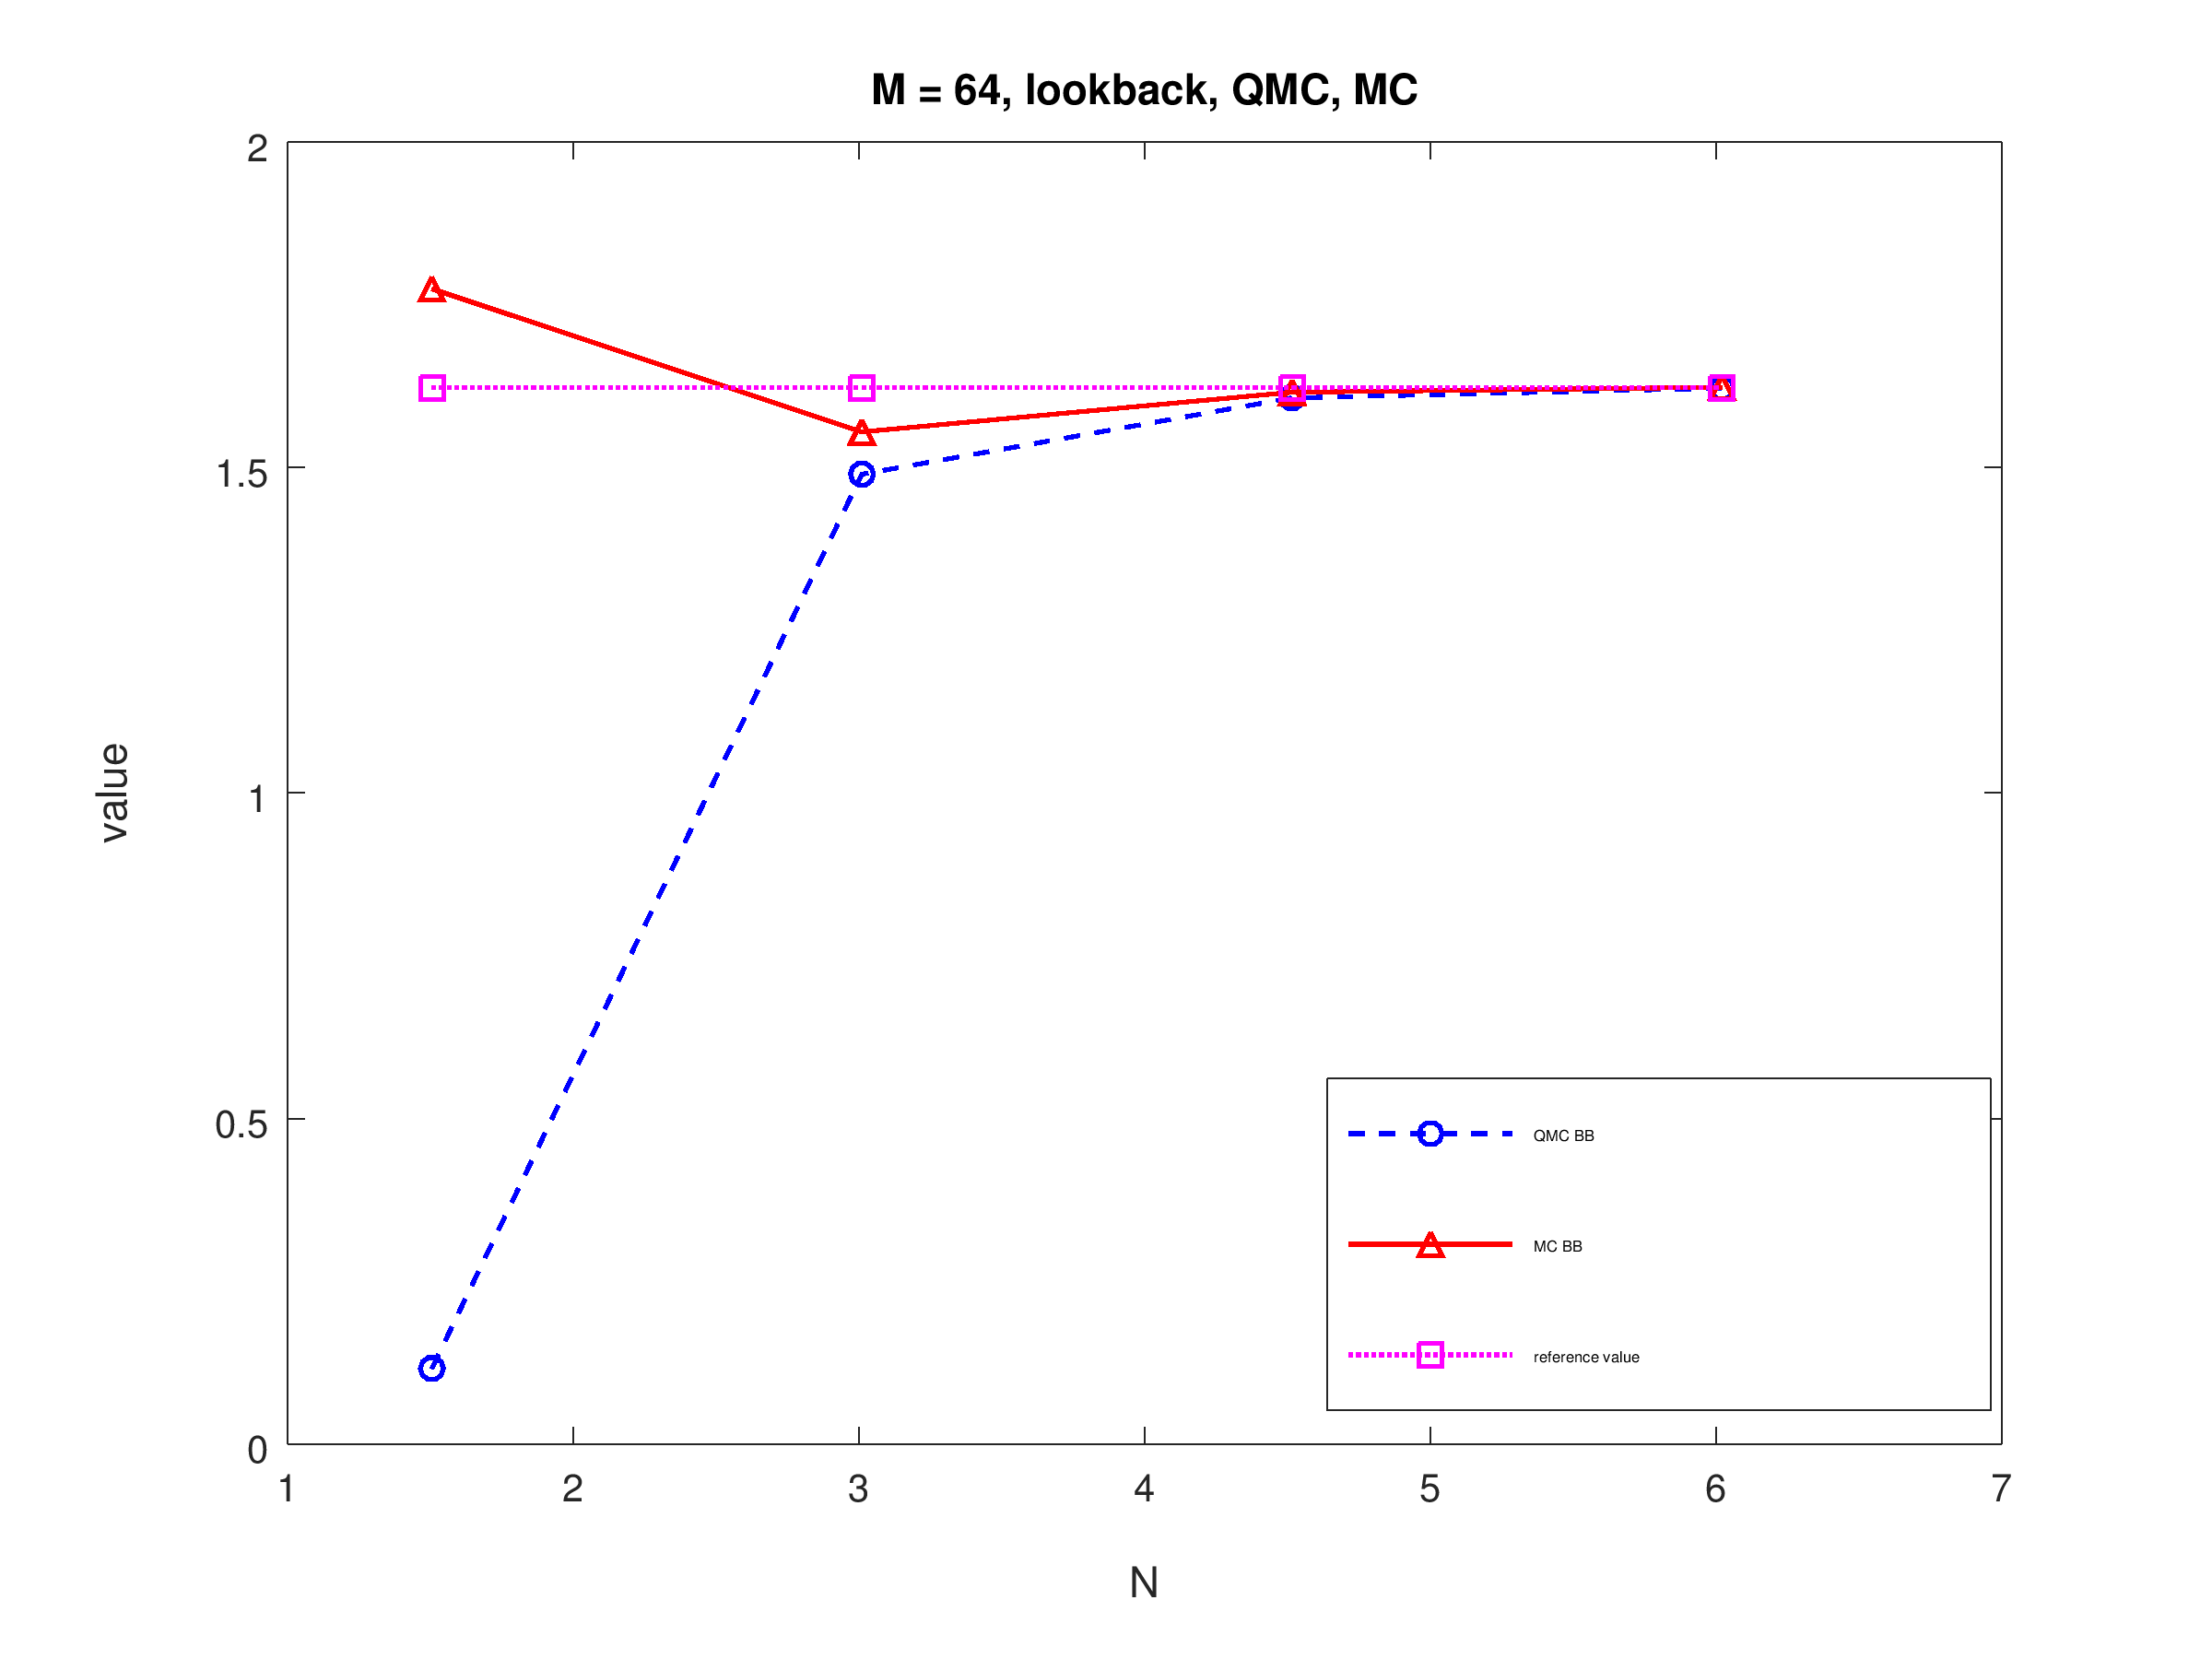
\includegraphics[scale=0.35]{../image/task6.png}
\end{center}
\begin{itemize}
    \item{
        On this figure value of lookback call option computed with QMC and MC methods using Brownian-Bridge is plotted against number of points.
        
    }
     
\end{itemize}
Here, once more, error between reference value computed numerically and value computed with QMC and MC using Brownian-Bridge against number of points.
\begin{center}
	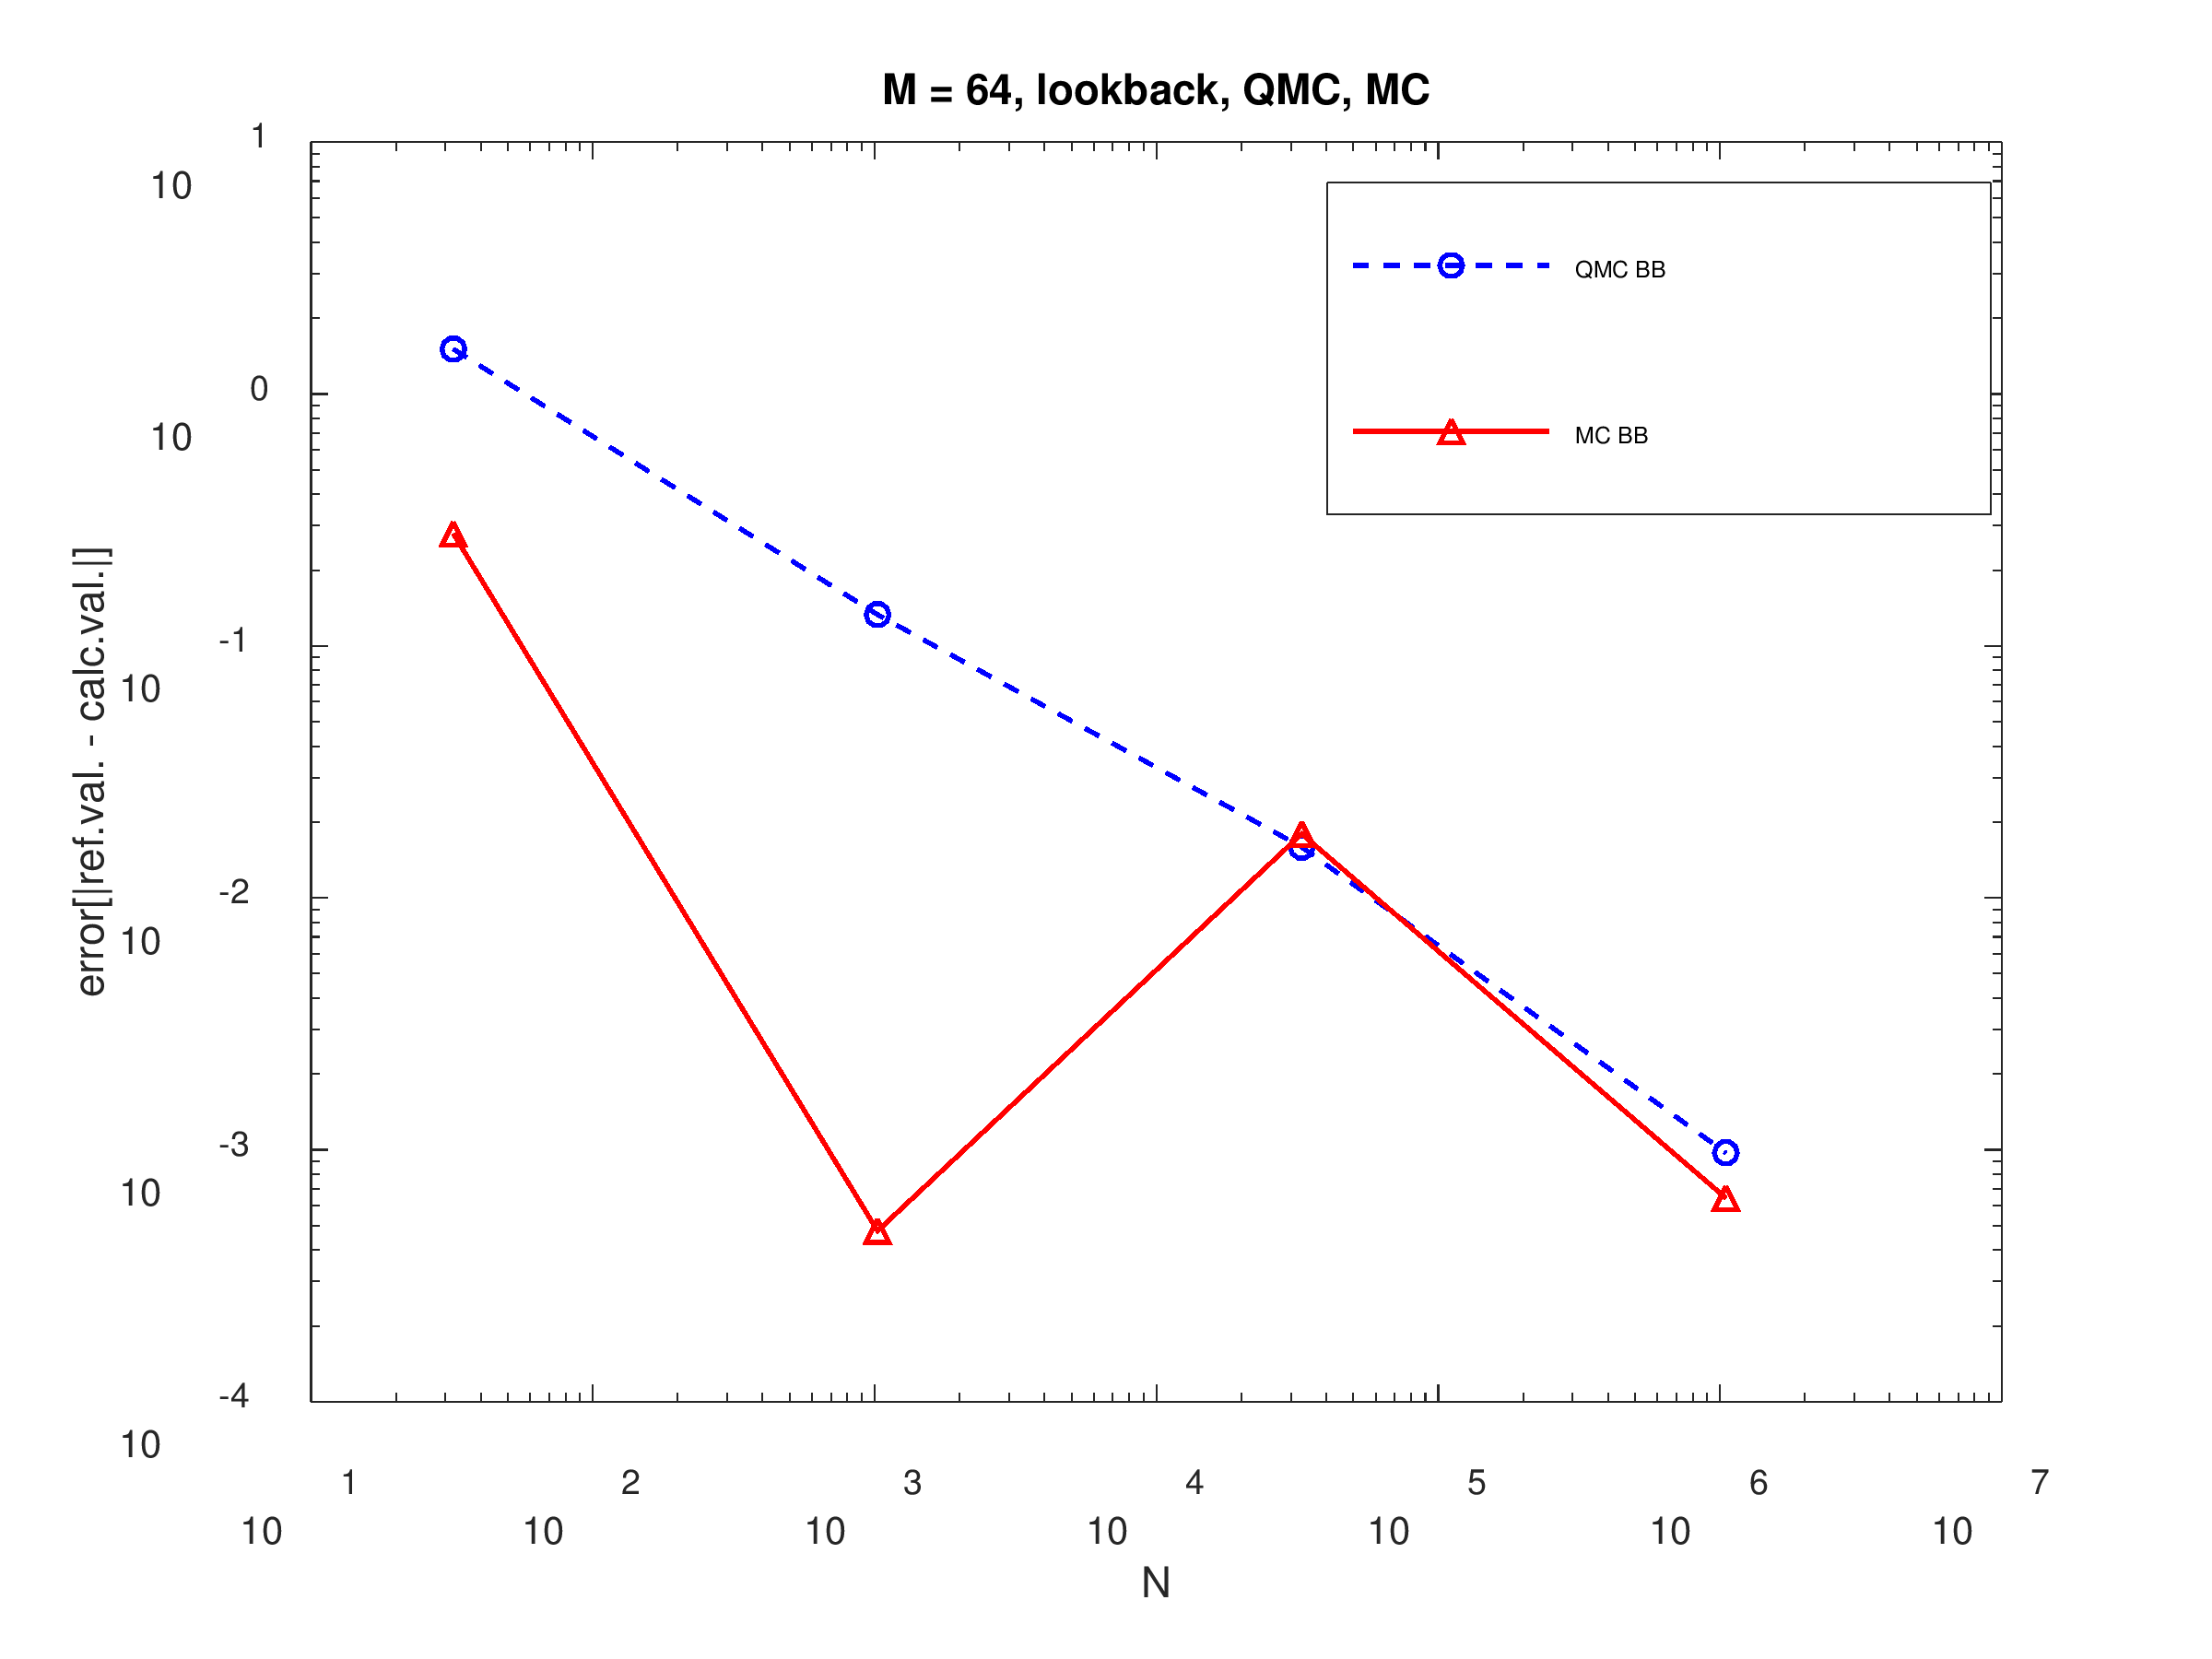
\includegraphics[scale=0.35]{../image/task6_error.png}
\end{center}

\section*{Task 7}


\begin{center}
	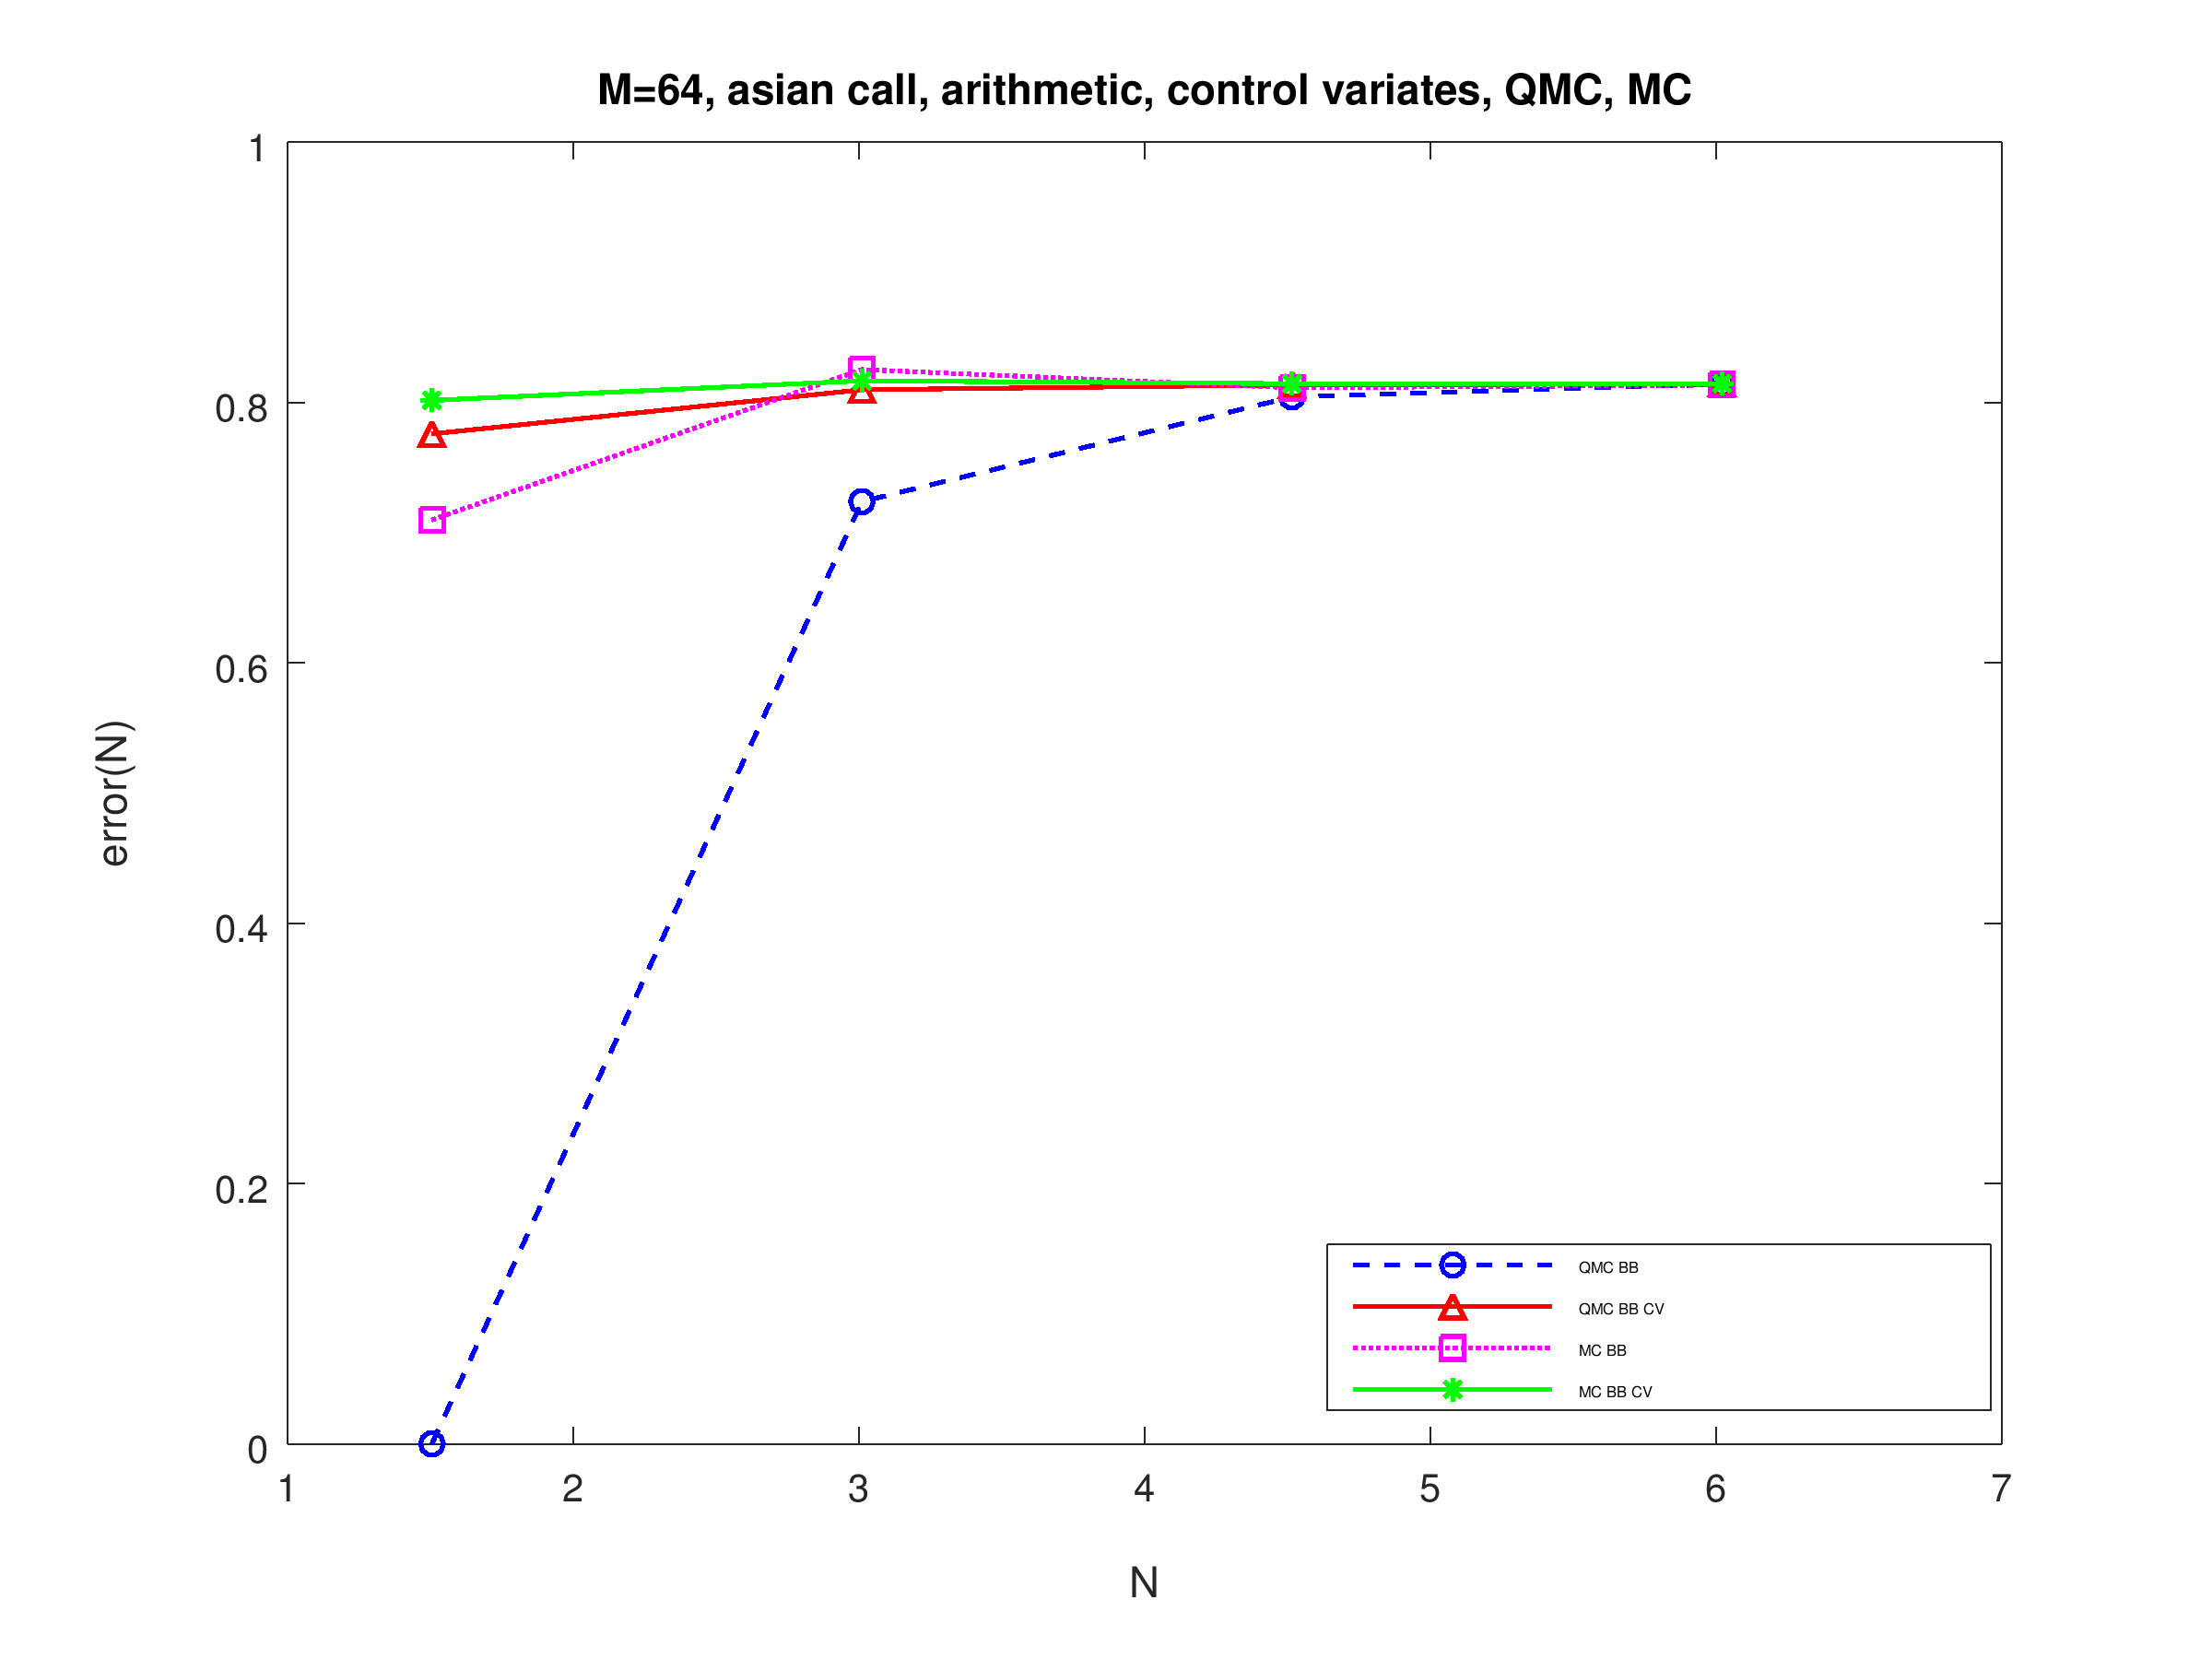
\includegraphics[scale=0.35]{../image/task7.png}
\end{center}
\begin{itemize}
    \item{
        On this figure, results of \textbf{control variates}
        method are presented. The idea was presented on the worksheet, but we observe, that this method improves slightly the variance in case of an arithmetic Asian call option. 
    }
\end{itemize}

\end{document}

